\documentclass[11pt]{article}
\usepackage{amsmath, amssymb}
\usepackage[pdftex]{graphicx}
\usepackage{subcaption}
\usepackage{units}
\usepackage{bm}
\usepackage{graphicx}
\usepackage[per-mode=symbol]{siunitx}
\usepackage[left=1in, right=1in, top=1in, bottom=1in]{geometry}
\usepackage{titling}

\title{Robot Learning : Maximum Entropy Assignment}
\author{Junhyeok Ahn}
\date{\today}
\begin{document}
\maketitle

%%%%%%%%%%%%%%%%%%%%%%%%%%%%%%%%%%%%%%%%%%%%%%%%%%%%%%%%%%%%%%%%%%%%%%%%%%%%%%
\section{Step Size}
Gradient descent algorithm usually require careful choice on step size. In the
beginning of the algorithm, large step is required for convergence rate however
small step size is required at the end. To choose step size, I used line search
algorithm. According to the paper, my object function and gradient could be
calculated as
\begin{equation}
    \begin{aligned}
        \label{eq:cost_and_grad}
        J(\bm{\theta}) &= \sum_{\tau \in D} \log P(\tau \mid \bm{\theta}) \\
        \triangledown_{\bm{\theta}}J(\bm{\theta}) &= \tilde{\mathbf{f}} - \sum_{s_i}D_{s_i} \mathbf{f}_{s_i}.
    \end{aligned}
\end{equation}
Once gradient is calculated, I updated new reward parameters with learning rate $\alpha$
and compute new reward as
\begin{equation}
    \begin{aligned}
        \label{eq:line_search}
        \theta_{\rm{new}} &= \bm{\theta} + \alpha \triangledown_{\bm{\theta}} \\
        J(\theta_{\rm{new}}) &= \sum_{\tau_{d} \in D} \log P(\tau_{d} \mid \theta_{\rm{new}}).
    \end{aligned}
\end{equation}
Then, I compared $J(\bm{\theta})$ and $J(\theta_{\rm{new}})$ and if the reward with new
parameters is higher, use step size $\alpha$ but if it is smaller, I reduced
step size half, so the reward could always increase.
\begin{figure}[htbp]
  \centering
  \begin{minipage}[b]{0.45\textwidth}
    \includegraphics[width=\textwidth]{figures/no_line_search.png}
    \caption{Use same stepsize 0.1 without adjustment}
  \end{minipage}
  \hfill
  \begin{minipage}[b]{0.45\textwidth}
    \includegraphics[width=\textwidth]{figures/line_search.png}
    \caption{Stepsize adjustment using line search}
  \end{minipage}
\end{figure}
In the attached code, I put line search algorithm right after the gradient
computation.

\section{100 Epochs with a Horizon of 10}
\label{sec:100_epochs_with_a_horizon_of_10}
I run the Maxent algorithm with 100 epochs and a horizon of 10 with line search
algorithm described in the previous problem to adjust step size. The graph of
\begin{figure}[htpb]
    \centering
    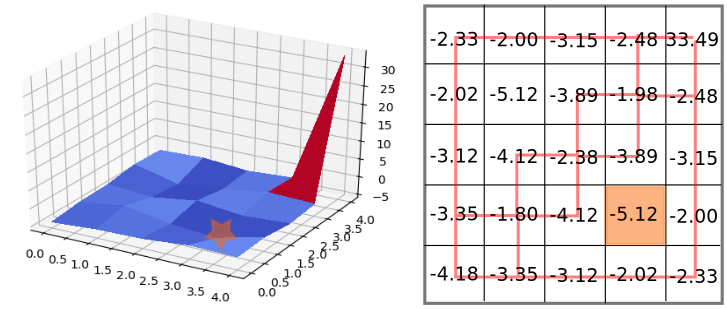
\includegraphics[width=0.8\linewidth]{figures/reward.png}
    \caption{Reward function with 100 epochs and horizon of 10 with line search.
            Orange cell represent state 8 which is an obstacle.}
    \label{fig:figures/reward}
\end{figure}
reward function is shown in Figure~\ref{fig:figures/reward}. Overally, it shows
significantly high reward at state 24 or $(4,4)$ and shows low reward at other states
relatively. Since the demonstrations gvien was intentionally trying to
avoid state 8 or $(1,3)$, the reward at there is especially low. One thing interesting
is that the reward function is symmetry because the given demonstrations are
symmetry. That is why state 16 or $(3,1)$ is as low as state 8 and the reward
seems to tell state 16 should be also avoided.
\begin{figure}[htpb]
    \centering
    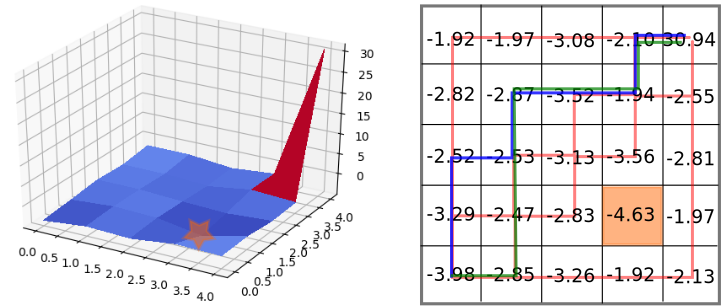
\includegraphics[width=0.8\linewidth]{figures/reward1.png}
    \caption{Reward function with 100 epochs and horizon of 10 with line search.
        Blue [0,5,10,11,16,17,18,23,24,25] and green [0,1,6,11,16,21,22,23,24,25] demonstrations are added to prevent underfitting.
            Orange cell represent state 8 which is an obstacle.}
    \label{fig:reward1}
\end{figure}

I think this result is underfitted because in order to represent
demonstrations' behavior (try to avoid state 8), reward function 16 is
incorrectly induced.  To prevent underfitting, we should provide more
demonstration around safe regions.  In Figure~\ref{fig:reward1}, I added two
more green and blue demonstrations to give more information about reward
function. In the attached, at the beginning of the algorithm I appended two
more demonstration.

\section{Derivation of Gradient}
\label{sec:derivation_of_gradient}
The purpose of Maxent algorithm is to find reward parameters and could be formulated
as below.
\begin{equation}
    \begin{aligned}
        \label{eq:grad_calc_1}
        \bm{\theta}^{\ast} &= \rm{argmax}_{\bm{\theta}} \sum_{\tau_{d} \in D} \log P(\tau_{d} \mid \bm{\theta}), \\
                    &= \rm{argmax}_{\bm{\theta}} \frac{1}{M}\sum_{\tau_{d} \in D} \log \frac{e^{r(\tau)}}{Z}, \\
                    &= \rm{argmax}_{\bm{\theta}} \frac{1}{M}\sum_{\tau_{d} \in D} r(\tau) - \log{Z}, \\
    \end{aligned}
\end{equation}
where M is the number of demonstration trajectories, $r(\tau)=\sum_{s \in \tau} \bm{\theta}^\top \mathbf{f}(s)$
and $Z=\sum_{\tau \in D} e^{r({\tau})}$.
Then,
\begin{equation}
    \begin{aligned}
        \label{eq:grad_calc_2}
        \bm{\theta}^{\ast} &= \rm{argmax}_{\bm{\theta}} \frac{1}{M} \sum_{\tau \in D} r(\tau) - \log \sum_{\tau \in D} e^{r(\tau)}, \\
                           &= \rm{argmax}_{\bm{\theta}} \frac{1}{M} \sum_{\tau \in D} \bm{\theta}^{\top} \mathbf{f}_{\tau} - \log \sum_{\tau \in D} e^{\bm{\theta}^{\top}\mathbf{f}_{\tau}}.
    \end{aligned}
\end{equation}
It is able to see the convexity of object function, which could be taken derivative as
\begin{equation}
    \begin{aligned}
        \label{eq:grad_calc_3}
        \triangledown_{\bm{\theta}}J &= \frac{1}{M} \sum_{\tau \in D} \mathbf{f}_{\tau} - \frac{1}{\sum_{\tau}e^{r(\tau)}} \sum_{\tau} e^{r(\tau) \frac{dr(\tau)}{d \bm{\theta}}}, \\
                                     &= \frac{1}{M} \sum_{\tau \in D} \mathbf{f}_{\tau} - \sum_{\tau \in D} \frac{e^{r(\tau)}}{\sum_{\tau}e^{r(\tau)}}\mathbf{f}_{\tau}, \\
                                     &= \frac{1}{M} \sum_{\tau \in D} \mathbf{f}_{\tau} - \sum_{\tau \in D} P(\tau \mid \theta)\mathbf{f}_{\tau}, \\
                                     &= \tilde{\mathbf{f}} - \sum_{s} D_{s}\mathbf{f}_{s},
    \end{aligned}
\end{equation}
where $\tilde{\mathbf{f}}=\frac{1}{M} \sum_{\tau \in D} \mathbf{f}_{\tau}$ and $D_{s}\mathbf{f}_{s}$ is state visitation frequency for state s.

\section{Different between Maxent algorithm and Action Based Distribution model}
\label{sec:4}
Intuitevely Maxent algorithm (Eq.(5) in the paper) computes probability of an
action as the expectation of exponentiated rewards of all path that start with
the action. For example in Figure~\ref{fig:figures/prob3}, when compute for $P(\uparrow \mid
s_{\rm start})$, Maxent considers all possible path candidates (e.g. passing through (1) and
(2)) after taking action $\uparrow$. As a result, Maxent algorithm regards
taking action $\uparrow$ or $\rightarrow$ at starting state in
Figure~\ref{fig:figures/prob3} as same probability.

\begin{figure}[htpb]
    \centering
    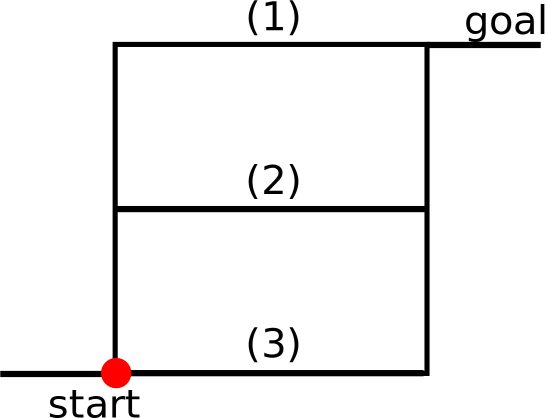
\includegraphics[width=0.4\linewidth]{figures/prob3.png}
    \caption{Example of probability distribution over paths}
    \label{fig:figures/prob3}
\end{figure}

However, action based model (Eq.(7) in the paper) computes action probability
as the expectation of exponentiated reward of a optimal path induced from
policy after taking the action. For example in Figure~\ref{fig:figures/prob3},
$P(\uparrow \mid s_{\rm start})$ is distributed based on the best reward of the
best policy after taking action $\uparrow$ (e.g. passing through (2)).
Therefore, although taking $\rightarrow$ or $\uparrow$ should yield same reward
and is supposed to be the same probability, action based model shows some bias
due to the action level probability mass.

This biased weight is problematic because it does not represent reward function
and violates the main assumption in the paper that if the reward of trajectory is same,
the probability is also same

\section{$Z_{a_{i,j}}$ and $Z_{s_i}$}
\label{sec:_z__a__ij_and_z__s_i_}

If we only have one terminal state and set the probability of being ended up at
terminal state is 1, recursively computed $Z_{a_{i,j}}$ represents the
occupancy associated state i when action j is taken (how much action j at state
i contributes to arrival of terminal state). It can be seen similar to
state-action value in terms of being described for each actions at each states.
Moreover, $Z_{s_i}$ is computed adding up all $Z_{a_{i,j}}$'s which are state
action values and could be interpreted as in trajectory how much portion $s_i$
is taking charge of given reward parameters. Therefore, the paper calculates
the policy by dividing each actions occupancy with total occupancy at state.

\section{Set $Z_{s}$ as Zero for Terminal State}
\label{sec:_z__s_set_to_zero_for_terminal_state}
\subsection{}
\label{sub:1}

As I mentioned in problem~\ref{sec:_z__a__ij_and_z__s_i_}, $Z_{a_{i,j}}$ and
$Z_{s_i}$ are backpropagated every iterations and represent how each states and
actions contribute to being ended at the terminal state. In this case, there is
only one terminal state and all trajectoried should be terminated at there. In
this perspective, $Z_s$ at terminal state should be set as 1. If we have two
 different equally distributed terminal states, they should be 0.5 each.

\subsection{}
\label{sub:2}

Reward at terminal state is always zero and the transition probability is
zeros.  Therefore, $Z_{a{i,j}}$ and $Z_{s_i}$ at terminal state ends up being
computed as zeros at each iteration. Therefore $Z_{s}$ at terminal should reset
to one at each iteration to represent the reward of being at terminal state.




\end{document}

